\documentclass{standalone}
\usepackage{tikz}
\usetikzlibrary{patterns, positioning}


\begin{document}
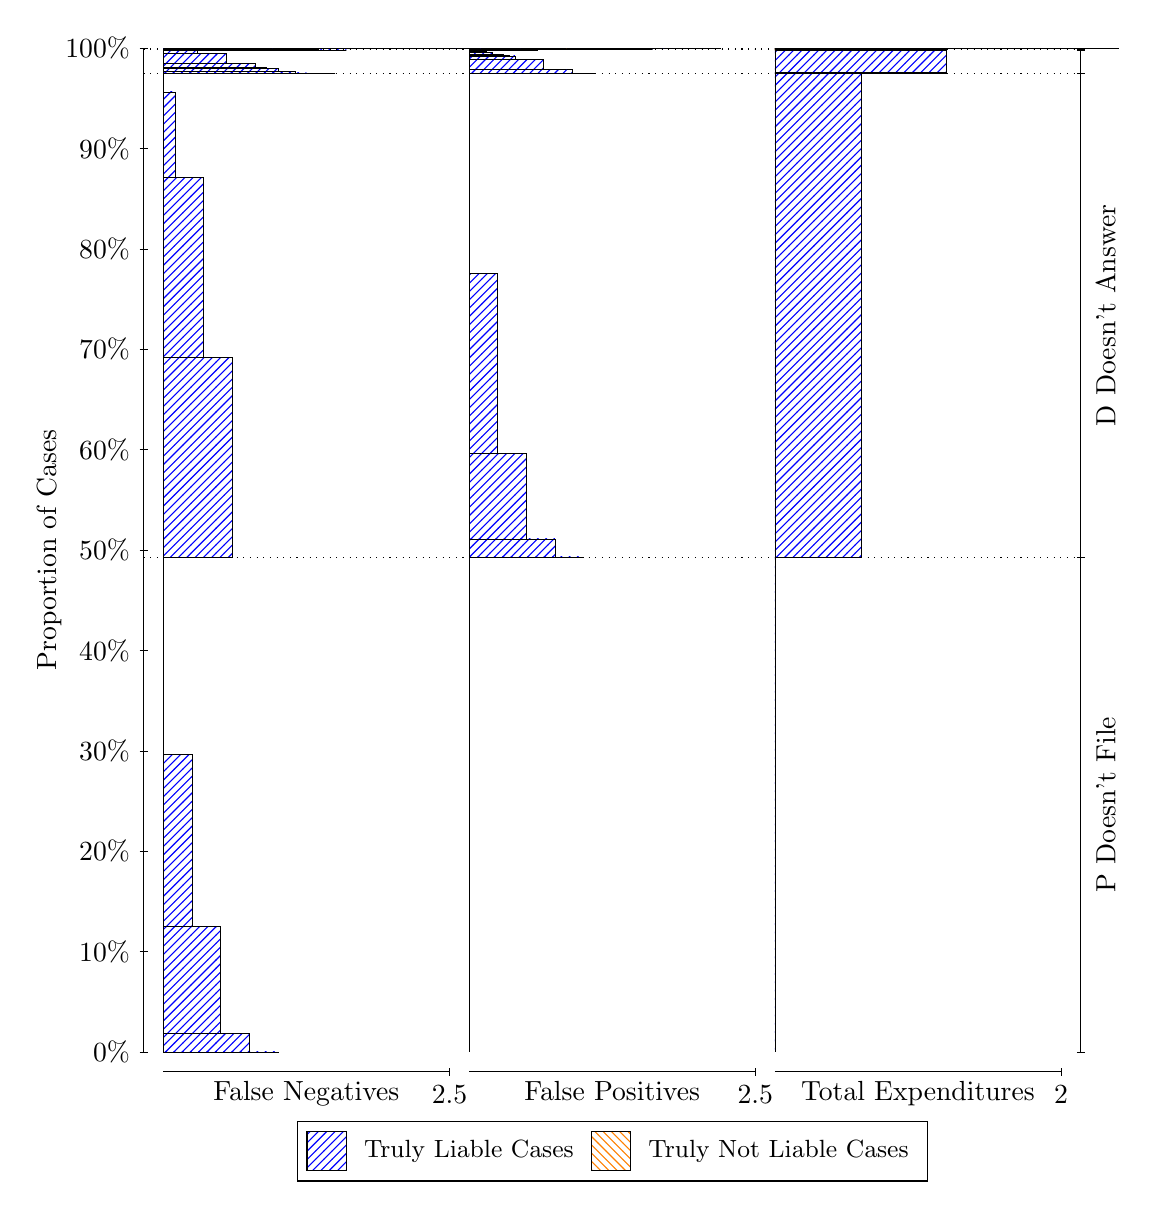
\begin{tikzpicture}
\draw[black, very thin] (1.5,1.75) -- (1.5,14.5);
\node[rotate=90, text=black, anchor=center] at (0.3, 8.125) {Proportion of Cases};
\draw[black, very thin] (1.45,1.75) -- (1.55,1.75);
\node[text=black, anchor=east] at (1.45, 1.75) {0\%};
\draw[black, very thin] (1.45,3.025) -- (1.55,3.025);
\node[text=black, anchor=east] at (1.45, 3.025) {10\%};
\draw[black, very thin] (1.45,4.3) -- (1.55,4.3);
\node[text=black, anchor=east] at (1.45, 4.3) {20\%};
\draw[black, very thin] (1.45,5.575) -- (1.55,5.575);
\node[text=black, anchor=east] at (1.45, 5.575) {30\%};
\draw[black, very thin] (1.45,6.85) -- (1.55,6.85);
\node[text=black, anchor=east] at (1.45, 6.85) {40\%};
\draw[black, very thin] (1.45,8.125) -- (1.55,8.125);
\node[text=black, anchor=east] at (1.45, 8.125) {50\%};
\draw[black, very thin] (1.45,9.4) -- (1.55,9.4);
\node[text=black, anchor=east] at (1.45, 9.4) {60\%};
\draw[black, very thin] (1.45,10.675) -- (1.55,10.675);
\node[text=black, anchor=east] at (1.45, 10.675) {70\%};
\draw[black, very thin] (1.45,11.95) -- (1.55,11.95);
\node[text=black, anchor=east] at (1.45, 11.95) {80\%};
\draw[black, very thin] (1.45,13.225) -- (1.55,13.225);
\node[text=black, anchor=east] at (1.45, 13.225) {90\%};
\draw[black, very thin] (1.45,14.5) -- (1.55,14.5);
\node[text=black, anchor=east] at (1.45, 14.5) {100\%};

\draw[black, very thin] (13.4,1.75) -- (13.4,14.5);
\draw[black, very thin] (13.35,1.75) -- (13.45,1.75);
\node[anchor=west] at (13.35, 1.75) {};
\draw[black, very thin] (13.35,8.0292) -- (13.45,8.0292);
\node[anchor=west] at (13.35, 8.0292) {};
\draw[black, very thin] (13.35,14.182) -- (13.45,14.182);
\node[anchor=west] at (13.35, 14.182) {};
\draw[black, very thin] (13.35,14.477) -- (13.45,14.477);
\node[anchor=west] at (13.35, 14.477) {};
\draw[black, very thin] (13.35,14.484) -- (13.45,14.484);
\node[anchor=west] at (13.35, 14.484) {};
\draw[black, very thin] (13.35,14.499) -- (13.45,14.499);
\node[anchor=west] at (13.35, 14.499) {};
\draw[black, very thin] (13.35,14.5) -- (13.45,14.5);
\node[anchor=west] at (13.35, 14.5) {};

\draw[black, very thin, pattern color=blue, pattern=north east lines] (1.75,1.75) rectangle (3.2033,1.7523);
\draw[black, very thin, pattern color=blue, pattern=north east lines] (1.75,1.7523) rectangle (2.84,1.985);
\draw[black, very thin, pattern color=blue, pattern=north east lines] (1.75,1.985) rectangle (2.4767,3.3418);
\draw[black, very thin, pattern color=blue, pattern=north east lines] (1.75,3.3418) rectangle (2.1133,5.5315);
\draw[black, very thin, pattern color=orange, pattern=north west lines] (1.75,5.5315) rectangle (1.75,5.5315);
\draw[black, very thin, pattern color=blue, pattern=north east lines] (1.75,5.5315) rectangle (1.75,8.0292);
\draw[black, very thin, pattern color=blue, pattern=north east lines] (1.75,8.0292) rectangle (2.622,10.576);
\draw[black, very thin, pattern color=blue, pattern=north east lines] (1.75,10.576) rectangle (2.2587,12.859);
\draw[black, very thin, pattern color=blue, pattern=north east lines] (1.75,12.859) rectangle (1.8953,13.944);
\draw[black, very thin, pattern color=orange, pattern=north west lines] (1.75,13.944) rectangle (1.75,13.944);
\draw[black, very thin, pattern color=blue, pattern=north east lines] (1.75,13.944) rectangle (1.75,14.182);
\draw[black, very thin, pattern color=blue, pattern=north east lines] (1.75,14.182) rectangle (3.93,14.182);
\draw[black, very thin, pattern color=blue, pattern=north east lines] (1.75,14.182) rectangle (3.7847,14.182);
\draw[black, very thin, pattern color=blue, pattern=north east lines] (1.75,14.182) rectangle (3.6393,14.182);
\draw[black, very thin, pattern color=blue, pattern=north east lines] (1.75,14.182) rectangle (3.5667,14.185);
\draw[black, very thin, pattern color=blue, pattern=north east lines] (1.75,14.185) rectangle (3.4213,14.201);
\draw[black, very thin, pattern color=blue, pattern=north east lines] (1.75,14.201) rectangle (3.3487,14.201);
\draw[black, very thin, pattern color=blue, pattern=north east lines] (1.75,14.201) rectangle (3.276,14.207);
\draw[black, very thin, pattern color=blue, pattern=north east lines] (1.75,14.207) rectangle (3.2033,14.238);
\draw[black, very thin, pattern color=blue, pattern=north east lines] (1.75,14.238) rectangle (3.058,14.255);
\draw[black, very thin, pattern color=blue, pattern=north east lines] (1.75,14.255) rectangle (2.9853,14.259);
\draw[black, very thin, pattern color=blue, pattern=north east lines] (1.75,14.259) rectangle (2.9127,14.301);
\draw[black, very thin, pattern color=blue, pattern=north east lines] (1.75,14.301) rectangle (2.84,14.302);
\draw[black, very thin, pattern color=blue, pattern=north east lines] (1.75,14.302) rectangle (2.6947,14.302);
\draw[black, very thin, pattern color=blue, pattern=north east lines] (1.75,14.302) rectangle (2.622,14.304);
\draw[black, very thin, pattern color=blue, pattern=north east lines] (1.75,14.304) rectangle (2.5493,14.432);
\draw[black, very thin, pattern color=blue, pattern=north east lines] (1.75,14.432) rectangle (2.4767,14.432);
\draw[black, very thin, pattern color=blue, pattern=north east lines] (1.75,14.432) rectangle (2.3313,14.432);
\draw[black, very thin, pattern color=blue, pattern=north east lines] (1.75,14.432) rectangle (2.2587,14.432);
\draw[black, very thin, pattern color=blue, pattern=north east lines] (1.75,14.432) rectangle (2.186,14.477);
\draw[black, very thin, pattern color=blue, pattern=north east lines] (1.75,14.477) rectangle (1.8953,14.477);
\draw[black, very thin, pattern color=orange, pattern=north west lines] (1.75,14.477) rectangle (1.75,14.477);
\draw[black, very thin, pattern color=blue, pattern=north east lines] (1.75,14.477) rectangle (4.0753,14.477);
\draw[black, very thin, pattern color=blue, pattern=north east lines] (1.75,14.477) rectangle (3.712,14.478);
\draw[black, very thin, pattern color=blue, pattern=north east lines] (1.75,14.478) rectangle (3.3487,14.484);
\draw[black, very thin, pattern color=blue, pattern=north east lines] (1.75,14.484) rectangle (2.9853,14.484);
\draw[black, very thin, pattern color=blue, pattern=north east lines] (1.75,14.484) rectangle (2.622,14.484);
\draw[black, very thin, pattern color=orange, pattern=north west lines] (1.75,14.484) rectangle (1.75,14.484);
\draw[black, very thin, pattern color=blue, pattern=north east lines] (1.75,14.484) rectangle (2.622,14.485);
\draw[black, very thin, pattern color=blue, pattern=north east lines] (1.75,14.485) rectangle (2.2587,14.49);
\draw[black, very thin, pattern color=blue, pattern=north east lines] (1.75,14.49) rectangle (1.8953,14.498);
\draw[black, very thin, pattern color=orange, pattern=north west lines] (1.75,14.498) rectangle (1.75,14.498);
\draw[black, very thin, pattern color=blue, pattern=north east lines] (1.75,14.498) rectangle (1.75,14.499);
\draw[black, very thin, pattern color=blue, pattern=north east lines] (1.75,14.499) rectangle (5.8193,14.499);
\draw[black, very thin, pattern color=blue, pattern=north east lines] (1.75,14.499) rectangle (5.456,14.499);
\draw[black, very thin, pattern color=blue, pattern=north east lines] (1.75,14.499) rectangle (5.0927,14.499);
\draw[black, very thin, pattern color=blue, pattern=north east lines] (1.75,14.499) rectangle (4.7293,14.499);
\draw[black, very thin, pattern color=blue, pattern=north east lines] (1.75,14.499) rectangle (4.584,14.499);
\draw[black, very thin, pattern color=blue, pattern=north east lines] (1.75,14.499) rectangle (4.366,14.499);
\draw[black, very thin, pattern color=blue, pattern=north east lines] (1.75,14.499) rectangle (4.2207,14.499);
\draw[black, very thin, pattern color=blue, pattern=north east lines] (1.75,14.499) rectangle (4.0027,14.499);
\draw[black, very thin, pattern color=blue, pattern=north east lines] (1.75,14.499) rectangle (3.8573,14.499);
\draw[black, very thin, pattern color=blue, pattern=north east lines] (1.75,14.499) rectangle (3.494,14.5);
\draw[black, very thin, pattern color=blue, pattern=north east lines] (1.75,14.5) rectangle (3.1307,14.5);
\draw[black, very thin, pattern color=blue, pattern=north east lines] (1.75,14.5) rectangle (2.7673,14.5);
\draw[black, very thin, pattern color=blue, pattern=north east lines] (1.75,14.5) rectangle (2.404,14.5);
\draw[black, very thin, pattern color=blue, pattern=north east lines] (1.75,14.5) rectangle (2.0407,14.5);
\draw[black, very thin, pattern color=orange, pattern=north west lines] (1.75,14.5) rectangle (1.75,14.5);
\draw[black, very thin, pattern color=orange, pattern=north west lines] (5.6333,1.75) rectangle (5.6333,1.75);
\draw[black, very thin, pattern color=blue, pattern=north east lines] (5.6333,1.75) rectangle (5.6333,8.0292);
\draw[black, very thin, pattern color=orange, pattern=north west lines] (5.6333,8.0292) rectangle (7.0867,8.0292);
\draw[black, very thin, pattern color=blue, pattern=north east lines] (5.6333,8.0292) rectangle (7.0867,8.0362);
\draw[black, very thin, pattern color=blue, pattern=north east lines] (5.6333,8.0362) rectangle (6.7233,8.2672);
\draw[black, very thin, pattern color=blue, pattern=north east lines] (5.6333,8.2672) rectangle (6.36,9.3518);
\draw[black, very thin, pattern color=blue, pattern=north east lines] (5.6333,9.3518) rectangle (5.9967,11.635);
\draw[black, very thin, pattern color=blue, pattern=north east lines] (5.6333,11.635) rectangle (5.6333,14.182);
\draw[black, very thin, pattern color=orange, pattern=north west lines] (5.6333,14.182) rectangle (7.232,14.182);
\draw[black, very thin, pattern color=blue, pattern=north east lines] (5.6333,14.182) rectangle (7.232,14.182);
\draw[black, very thin, pattern color=orange, pattern=north west lines] (5.6333,14.182) rectangle (6.9413,14.182);
\draw[black, very thin, pattern color=blue, pattern=north east lines] (5.6333,14.182) rectangle (6.9413,14.227);
\draw[black, very thin, pattern color=blue, pattern=north east lines] (5.6333,14.227) rectangle (6.8687,14.227);
\draw[black, very thin, pattern color=orange, pattern=north west lines] (5.6333,14.227) rectangle (6.796,14.227);
\draw[black, very thin, pattern color=blue, pattern=north east lines] (5.6333,14.227) rectangle (6.796,14.227);
\draw[black, very thin, pattern color=orange, pattern=north west lines] (5.6333,14.227) rectangle (6.6507,14.227);
\draw[black, very thin, pattern color=blue, pattern=north east lines] (5.6333,14.227) rectangle (6.6507,14.227);
\draw[black, very thin, pattern color=blue, pattern=north east lines] (5.6333,14.227) rectangle (6.578,14.354);
\draw[black, very thin, pattern color=blue, pattern=north east lines] (5.6333,14.354) rectangle (6.5053,14.356);
\draw[black, very thin, pattern color=blue, pattern=north east lines] (5.6333,14.356) rectangle (6.4327,14.356);
\draw[black, very thin, pattern color=blue, pattern=north east lines] (5.6333,14.356) rectangle (6.2873,14.358);
\draw[black, very thin, pattern color=blue, pattern=north east lines] (5.6333,14.358) rectangle (6.2147,14.4);
\draw[black, very thin, pattern color=blue, pattern=north east lines] (5.6333,14.4) rectangle (6.142,14.403);
\draw[black, very thin, pattern color=blue, pattern=north east lines] (5.6333,14.403) rectangle (6.0693,14.42);
\draw[black, very thin, pattern color=blue, pattern=north east lines] (5.6333,14.42) rectangle (5.924,14.452);
\draw[black, very thin, pattern color=blue, pattern=north east lines] (5.6333,14.452) rectangle (5.8513,14.457);
\draw[black, very thin, pattern color=blue, pattern=north east lines] (5.6333,14.457) rectangle (5.7787,14.457);
\draw[black, very thin, pattern color=blue, pattern=north east lines] (5.6333,14.457) rectangle (5.706,14.474);
\draw[black, very thin, pattern color=blue, pattern=north east lines] (5.6333,14.474) rectangle (5.6333,14.477);
\draw[black, very thin, pattern color=orange, pattern=north west lines] (5.6333,14.477) rectangle (6.5053,14.477);
\draw[black, very thin, pattern color=blue, pattern=north east lines] (5.6333,14.477) rectangle (6.5053,14.477);
\draw[black, very thin, pattern color=blue, pattern=north east lines] (5.6333,14.477) rectangle (6.142,14.477);
\draw[black, very thin, pattern color=blue, pattern=north east lines] (5.6333,14.477) rectangle (5.7787,14.484);
\draw[black, very thin, pattern color=blue, pattern=north east lines] (5.6333,14.484) rectangle (5.6333,14.484);
\draw[black, very thin, pattern color=orange, pattern=north west lines] (5.6333,14.484) rectangle (7.9587,14.484);
\draw[black, very thin, pattern color=blue, pattern=north east lines] (5.6333,14.484) rectangle (7.9587,14.484);
\draw[black, very thin, pattern color=blue, pattern=north east lines] (5.6333,14.484) rectangle (7.5953,14.485);
\draw[black, very thin, pattern color=blue, pattern=north east lines] (5.6333,14.485) rectangle (7.232,14.493);
\draw[black, very thin, pattern color=blue, pattern=north east lines] (5.6333,14.493) rectangle (6.8687,14.498);
\draw[black, very thin, pattern color=blue, pattern=north east lines] (5.6333,14.498) rectangle (6.5053,14.499);
\draw[black, very thin, pattern color=orange, pattern=north west lines] (5.6333,14.499) rectangle (8.8307,14.499);
\draw[black, very thin, pattern color=blue, pattern=north east lines] (5.6333,14.499) rectangle (8.8307,14.499);
\draw[black, very thin, pattern color=blue, pattern=north east lines] (5.6333,14.499) rectangle (8.4673,14.499);
\draw[black, very thin, pattern color=orange, pattern=north west lines] (5.6333,14.499) rectangle (8.4673,14.499);
\draw[black, very thin, pattern color=blue, pattern=north east lines] (5.6333,14.499) rectangle (8.4673,14.499);
\draw[black, very thin, pattern color=blue, pattern=north east lines] (5.6333,14.499) rectangle (8.104,14.499);
\draw[black, very thin, pattern color=orange, pattern=north west lines] (5.6333,14.499) rectangle (8.104,14.499);
\draw[black, very thin, pattern color=blue, pattern=north east lines] (5.6333,14.499) rectangle (8.104,14.499);
\draw[black, very thin, pattern color=blue, pattern=north east lines] (5.6333,14.499) rectangle (7.7407,14.499);
\draw[black, very thin, pattern color=orange, pattern=north west lines] (5.6333,14.499) rectangle (7.7407,14.499);
\draw[black, very thin, pattern color=blue, pattern=north east lines] (5.6333,14.499) rectangle (7.7407,14.499);
\draw[black, very thin, pattern color=blue, pattern=north east lines] (5.6333,14.499) rectangle (7.3773,14.499);
\draw[black, very thin, pattern color=blue, pattern=north east lines] (5.6333,14.499) rectangle (7.3773,14.5);
\draw[black, very thin, pattern color=blue, pattern=north east lines] (5.6333,14.5) rectangle (7.014,14.5);
\draw[black, very thin, pattern color=orange, pattern=north west lines] (5.6333,14.5) rectangle (6.8687,14.5);
\draw[black, very thin, pattern color=blue, pattern=north east lines] (5.6333,14.5) rectangle (6.8687,14.5);
\draw[black, very thin, pattern color=blue, pattern=north east lines] (5.6333,14.5) rectangle (6.6507,14.5);
\draw[black, very thin, pattern color=orange, pattern=north west lines] (5.6333,14.5) rectangle (6.5053,14.5);
\draw[black, very thin, pattern color=blue, pattern=north east lines] (5.6333,14.5) rectangle (6.5053,14.5);
\draw[black, very thin, pattern color=blue, pattern=north east lines] (5.6333,14.5) rectangle (6.2873,14.5);
\draw[black, very thin, pattern color=blue, pattern=north east lines] (5.6333,14.5) rectangle (6.142,14.5);
\draw[black, very thin, pattern color=blue, pattern=north east lines] (5.6333,14.5) rectangle (5.7787,14.5);
\draw[black, very thin, pattern color=blue, pattern=north east lines] (5.6333,14.5) rectangle (5.6333,14.5);
\draw[black, very thin, pattern color=orange, pattern=north west lines] (9.5167,1.75) rectangle (9.5167,1.75);
\draw[black, very thin, pattern color=blue, pattern=north east lines] (9.5167,1.75) rectangle (9.5167,8.0292);
\draw[black, very thin, pattern color=orange, pattern=north west lines] (9.5167,8.0292) rectangle (10.607,8.0292);
\draw[black, very thin, pattern color=blue, pattern=north east lines] (9.5167,8.0292) rectangle (10.607,14.182);
\draw[black, very thin, pattern color=orange, pattern=north west lines] (9.5167,14.182) rectangle (11.697,14.182);
\draw[black, very thin, pattern color=blue, pattern=north east lines] (9.5167,14.182) rectangle (11.697,14.187);
\draw[black, very thin, pattern color=orange, pattern=north west lines] (9.5167,14.187) rectangle (11.697,14.187);
\draw[black, very thin, pattern color=blue, pattern=north east lines] (9.5167,14.187) rectangle (11.697,14.477);
\draw[black, very thin, pattern color=orange, pattern=north west lines] (9.5167,14.477) rectangle (11.697,14.477);
\draw[black, very thin, pattern color=blue, pattern=north east lines] (9.5167,14.477) rectangle (11.697,14.484);
\draw[black, very thin, pattern color=orange, pattern=north west lines] (9.5167,14.484) rectangle (11.697,14.484);
\draw[black, very thin, pattern color=blue, pattern=north east lines] (9.5167,14.484) rectangle (11.697,14.499);
\draw[black, very thin, pattern color=orange, pattern=north west lines] (9.5167,14.499) rectangle (13.877,14.499);
\draw[black, very thin, pattern color=blue, pattern=north east lines] (9.5167,14.499) rectangle (13.877,14.499);
\draw[black, very thin, pattern color=orange, pattern=north west lines] (9.5167,14.499) rectangle (13.877,14.499);
\draw[black, very thin, pattern color=blue, pattern=north east lines] (9.5167,14.499) rectangle (13.877,14.5);
\draw[black, dotted] (1.5,8.0292) -- (13.4,8.0292);
\draw[black, dotted] (1.5,14.182) -- (13.4,14.182);
\draw[black, dotted] (1.5,14.477) -- (13.4,14.477);
\draw[black, dotted] (1.5,14.484) -- (13.4,14.484);
\draw[black, dotted] (1.5,14.499) -- (13.4,14.499);
\draw[black, very thin] (1.75,1.5) -- (5.3833,1.5);
\node[text=black, anchor=north] at (3.5667, 1.5) {False Negatives};
\draw[black, very thin] (5.3833,1.45) -- (5.3833,1.55);
\node[text=black, anchor=north] at (5.3833, 1.45) {2.5};

\draw[black, very thin] (5.6333,1.5) -- (9.2667,1.5);
\node[text=black, anchor=north] at (7.45, 1.5) {False Positives};
\draw[black, very thin] (9.2667,1.45) -- (9.2667,1.55);
\node[text=black, anchor=north] at (9.2667, 1.45) {2.5};

\draw[black, very thin] (9.5167,1.5) -- (13.15,1.5);
\node[text=black, anchor=north] at (11.333, 1.5) {Total Expenditures};
\draw[black, very thin] (13.15,1.45) -- (13.15,1.55);
\node[text=black, anchor=north] at (13.15, 1.45) {2};

\node[text=black, centered, rotate=90] at (13.72, 4.8896) {P Doesn't File};
\node[text=black, centered, rotate=90] at (13.72, 11.105) {D Doesn't Answer};





\draw (7.449999999999999,1.5) node[draw=none] (baseCoordinate) {};
\begin{scope}[align=center]
        \matrix[scale=0.5, draw=black, below=0.5cm of baseCoordinate, nodes={draw}, column sep=0.1cm]{
            \node[rectangle, draw, minimum width=0.5cm, minimum height=0.5cm, pattern color=blue, pattern=north east lines] {}; &
            \node[draw=none, font=\small, text=black] (B) {Truly Liable Cases}; &
            \node[rectangle, draw, minimum width=0.5cm, minimum height=0.5cm, pattern color=orange, pattern=north west lines] {}; &
            \node[draw=none, font=\small, text=black] (B) {Truly Not Liable Cases}; \\
            };
\end{scope}

\end{tikzpicture}
\end{document}